%!TeX root=../tese.tex
%(dica para o editor de texto: este arquivo é parte de um documento maior)
% para saber mais: https://tex.stackexchange.com/q/78101/183146

% https://otexts.com/fpp2/index.html
% https://www.tensorflow.org/tutorials/structured_data/time_series

\chapter{Séries temporais}
\label{cap:series}

Neste capítulo são apresentados os conceitos básicos de séries temporais. Também são discutidos brevemente os modelos tradicionais de análise e descrição das séries, ou de previsões de valores futuros, de acordo com o objetivo do estudo. Tais modelos são, por exemplo, baseados em médias móveis, tendências e sazonalidades presentes nos dados.

De acordo com Pedro A. Morettin e Clélia M C. Toloi \citep{morettin}, uma série temporal é qualquer conjunto de observações ordenadas no tempo. São exemplos: valores diários de poluição de uma cidade, valores mensais de temperatura, índices diários da bolsa de valores, número médio anual de manchas solares e registro de marés em portos e estuários.

A análise e predição de cotações de moedas estrangeiras, índices de ações, entre outros dados econômicos, constituem uma área essencial da economia e que exige a avaliação de um número enorme de fatores, muitos dos quais de características humanas e portanto imprevisíveis em sua exatidão, sendo descritos como exemplos de fenômenos \emph{estocásticos}, isto é, probabilísticos.

As séries temporais podem ser \defi{contínuas} em função do tempo, como é o exemplo de registros de marés, ou \defi{discretas} como são todos os outros exemplos, ou seja, os valores são tomados a $N$ intervalos regulares de um período $T$ considerado, tal que $N = T/\Delta t$. Na prática, para o uso em modelos, segundo explica Morettin e Toloi \citep{morettin}, as séries contínuas devem ser discretizadas em intervalos, uma vez que é esse tipo de dado que poderá ser processado num computador.

Pode-se classificar a análise das séries temporais de acordo com seu objetivo de estudo. Morettin e Toloi \citep{morettin} listam os alguns objetivos principais:

\begin{itemize}
	\item{Investigar o mecanismo gerador da série temporal, procurando descrevê-la a partir de uma função teórica.}
	\item{Fazer previsões de valores futuros da série, seja tanto a curto quanto a longo prazo.}
	\item{Descrição da série, em termos de tendências, variações sazonais, ou então análises descritivas por meio de histogramas, médias móveis, etc.}
	\item{Procurar por periodicidades relevantes nos dados, quando não fazemos suposições de periodicidades comuns como semanais, mensais ou anuais, por exemplo.}
\end{itemize}

Neste contexto, Morettin e Toloi \citep{morettin} definem que um modelo é uma descrição probabilística de uma série temporal, cabendo ao cientista de dados decidir a melhor utilização desse modelo segundo seus objetivos. 

Além disso eles afirmam que qualquer tarefa de previsão, sendo este o objetivo, será baseada em algum procedimento computacional que calcula uma estimativa do futuro baseada na otimização de uma função de perda a partir de combinações lineares de valores do passado. É a união de um modelo probabilístico com a otimização de uma função de perda que define um \defi{método de previsão}.

Há dois tipos básicos de modelos que lidam com séries temporais, de acordo com Morettin e Toloi \citep{morettin}, que são os modelos \defi{paramétricos}, onde a análise é feita no \emph{domínio temporal} com suposições e parâmetros a serem estimados, e os modelos \defi{não-paramétricos}, em que a análise é feita no \emph{domínio das frequências} com um enfoque mais descritivo e sem muitas suposições. Este capítulo explica a diferença e o exemplo da utilização dos dois tipos de modelos.

Dentre os modelos paramétricos, destacam-se os modelos \emph{ARIMA} (\emph{autorregressivos integrados de médias móveis}), disponíveis como bibliotecas das linguagens \eng{Python} e \eng{R}, enquanto que entre os modelos não-paramétricos destaca-se a \emph{análise espectral}, também denominada de \emph{análise de Fourier}, já que as ferramentas utilizadas são as transformadas de Fourier e suas variações.

Na última seção desse capítulo, uma estrutura de uma rede neural recorrente, implementada com a API Keras, é proposta como um modelo \defi{semiparamétrico}, ou seja, estimando parâmetros inerentes às redes neurais, mas não utilizando parâmetros ou suposições específicas sobre os dados, para a realização de previsões de valores futuros de séries temporais financeiras, com enfoque nas séries históricas de cotações de moedas estrangeiras.\footnote{Tais séries estão disponíveis para \eng{download} no site do Banco Central do Brasil: \url{https://www.bcb.gov.br/}}.

\section{Processos estocásticos}

De acordo com Morettin e Toloi \citep{morettin}, um \defi{processo estocástico} é uma familia $Z = \{ Z(t), t \in \mathcal{T} \}$, onde o conjunto $\mathcal{T}$ é normalmente tomado como $\mathcal{T} \subseteq \mathbb{Z}$ ou $\mathcal{T} \subseteq \mathbb{R}$, tal que, para cada $t \in \mathcal{T}$, $Z(t)$ é uma variável aleatória. 

Portanto, um processo estocástico é uma família de variáveis aleatórias reais $Z(t),\; t \in \mathcal{T}$, definidas num mesmo espaço de probabilidades $(\Omega, \mathcal{A}, \mathcal{P})$, e portanto $Z(t)$ é uma função de dois argumentos, isto é, $Z(t, \omega),\; t \in \mathcal{T},\; \omega \in \Omega$.

Para cada $t \in \mathcal{T}$ fixado, $Z(t, \omega)$ será uma v.a. com uma distribuição de probabilidades. Pode haver uma distribuição diferente para cada $t \in \mathcal{T}$, mas normalmente assume-se que é a mesma, conforme dito por Morettin e Toloi \citep{morettin}.

Por outro lado, para cada $\omega_i \in \Omega$ fixado, denotamos $Z(t, \omega_i)$ por $Z^{(i)}(t)$ como uma função de $t$, denominada de \defi{trajetória} do processo, ou simplesmente de \emph{série temporal}. Isto define uma série temporal como uma trajetória ou realização de um processo estocástico, o que pode ser melhor ilustrado pela Figura \ref{fig:trajetorias}, abaixo.

\begin{figure}[htb]
\centering
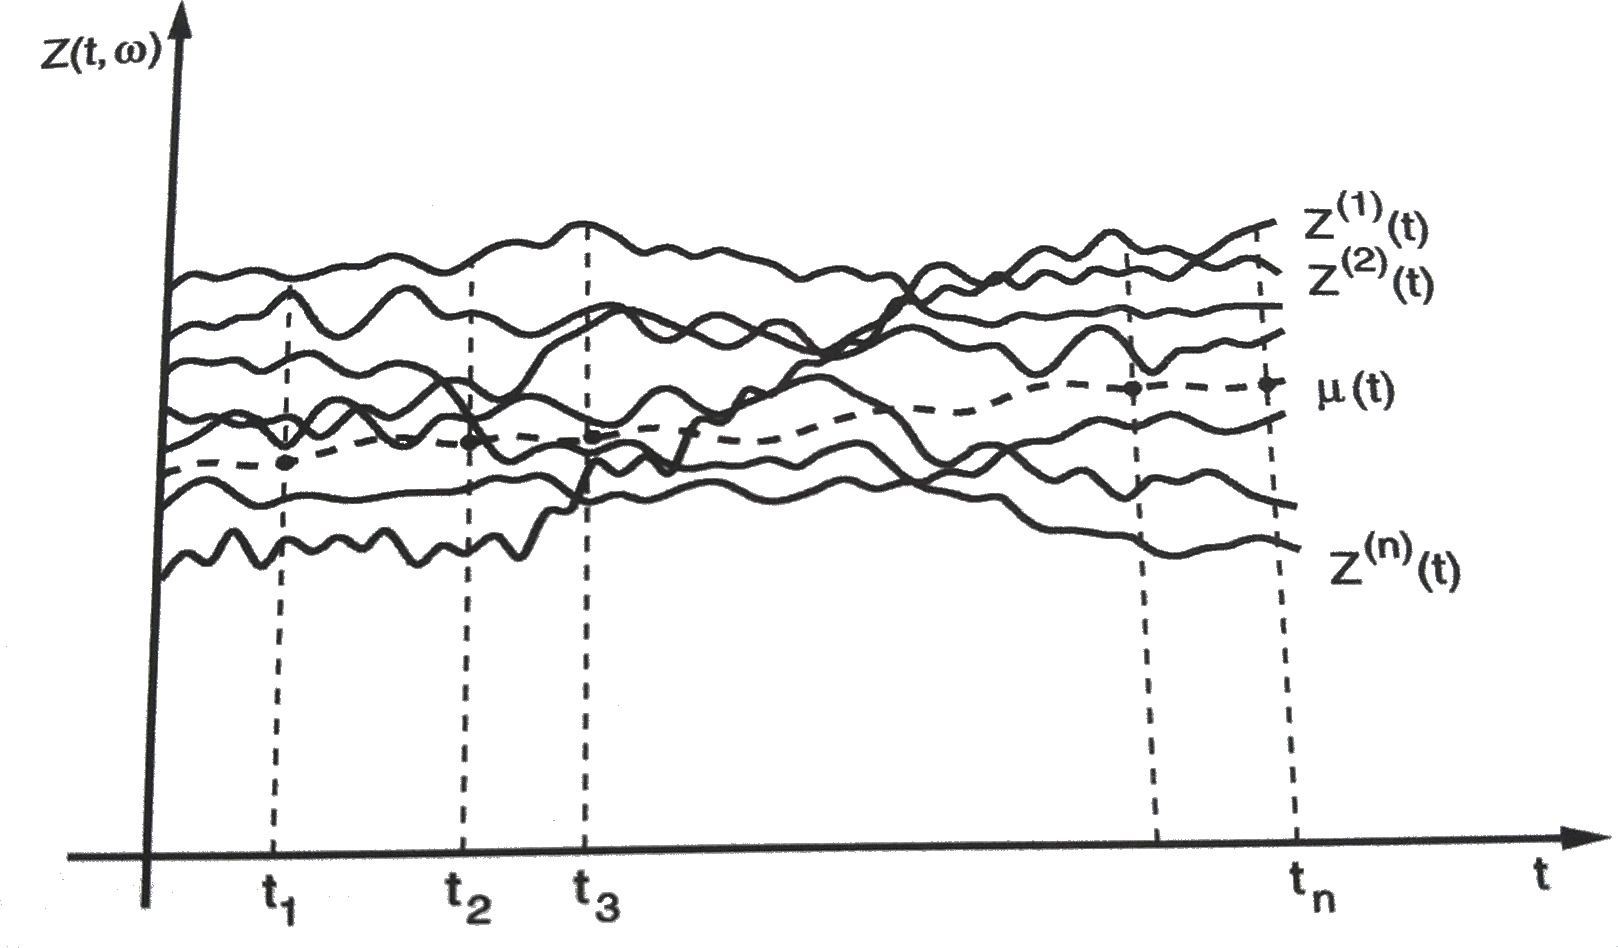
\includegraphics[width=10cm]{figuras/trajetorias}
\caption{Processo estocástico como uma família de trajetórias, isto é, de séries temporais.\footnote{Extraido de Morettin e Castro Toloi, 2019, pág 27.}}
\label{fig:trajetorias}
\end{figure}

\[ \mathcal{VOMITO} \]

\section{Modelos não-paramétricos: transformada de Fourier e a função de autocorrelação}

A transformada discreta de Fourier é uma função $2\pi$-periódica e definida em: \[F:(x_j)_{j \in \mathbb{N}} \rightarrow (z_j)_{j \in \mathbb{N}} \] onde $ x_j \in [0, 2\pi]$ e $ z_j \in C $, com $C \subset \mathbb{R}$ ou $C \subset \mathbb{C}$. Ou seja, é tabelada em $2N$ pontos igualmente espaçados (no caso das oscilações usamos os preços de cada dia, portanto levando a valores reais, e o intervalo de dias é o domínio), no intervalo $[0, 2\pi]$ (basta normalizar o intervalo de dias nesse intervalo, ou seja, denotando $x_j = j\pi/N $, com $j = 0, 1, \dots, 2N-1$). A função pode ser definida para um conjunto de pontos que podem ser complexos ou mesmo reais. Faz isso associando aos valores $F(x_j)$ os coeficientes de Fourier $(c_k)$, dessa forma:
\begin{equation}\label{tfd_1}
F(x_j) = \sum_{k=0}^{2N-1} c_k e^{ikx_j}\ ,\ j=0, 1, \dots, 2N-1
\end{equation}
\begin{equation}\label{tfd_2}
c_k = \frac{1}{2N} \sum_{j=0}^{2N-1} F(x_j) e^{-ikx_j}\ ,\ k=0, 1, \dots, 2N-1
\end{equation}

\section{Modelos paramétricos autoregressivos e de médias móveis}

\section{Um modelo semiparamétrico construído com uma rede neural}